\section{Einleitung}
\subsection{Relevanz des Themas}
Um im Rahmen der globalen Ausweitung wettbewerbsfähig zu bleiben, müssen sich Unternehmen ständig auf neue Herausforderungen einstellen. Dies erfordert eine hohe Reaktionsgeschwindigkeit des Managements und somit ein leistungsfähiges Berichtswesen, welches eine möglichst aktuelle Darstellung der Unternehmenslage ermöglicht. Um die Wirtschaftlichkeit zu steigern, ist es essentiell, in allen Unternehmensbereichen Kosten transparent zu erfassen und senken zu können. 
Die internationalen Märkte erfordern es, diese Unternehmensanforderungen mit facettenreichen, rechtlichen Auflagen unterschiedlichster Länder in Einklang zu bringen. 
Unabhängig von der Unternehmensgröße werden flexible IT-Systeme benötigt die ein optimales Unternehmenswachstum unterstützen.

Die SAP AG ist einer der weltweit führenden Anbieter für Unternehmenssoftware und gerade auf dem deutschen Markt, mit Ihren Produkten für das Rechnungswesen, ein bereits etablierter Standard\footnote{Vgl. \cite{Patel2009}, S. 21. f}.

 
%Viele Unternehmen sehen sich neuen Aufgabenstellungen gegen{\"u}ber. Ursache sind die Internationalisierung, die h{\"a}ufigen Produktwechsel und der Zwang zu permanenter\\Veränderung. Der Anteil der Routineaufgaben nimmt stetig ab, w{\"a}hrend andererseits neuartige und komplexer werdende Aufgaben anstehen\footnote{Vgl. \cite{Fiedler2008}, S.~1}.
%Die Durchführung dieser Aufgaben wird in der Unternehmenspraxis zunehmend in Form von Projekten vollzogen.
%Dass komplexe, neuartige und interdisziplinäre Projekte nicht intuitiv ausgewählt und zum Ziel geführt werden können, dürfte heute jedem Unternehmer klar sein.
%
%In diesem Zusammenhang treten facettenreiche und h{\"o}chst unterschiedliche Problemfelder auf, denen von Seiten der Unternehmenspraxis wie auch der Betriebswirtschaftslehre begegnet werden muss. Um eine geeignete Projektauswahl und Implementierung der Unternehmensstrategien in diese Projekte zu gewährleisten, muss die Unternehmensf{\"u}hrung und die Projektleitung durch eine sinnvolle und methodisch gepr{\"a}gte Planung und Kontrolle der Projekte eines Unternehmens unterst{\"u}tzt werden\footnote{Vgl. \cite{Kunz2007}, S.~1} \footnote{Vgl. \cite{Urli&Terrien2010}}.

\subsection{Zielsetzung und Abgrenzung}

%Diese Arbeit beschäftigt sich mit theorieorientierten Ausprägungen und Beschreibungen des Projektcontrollings. Das Thema wird in sinnvollen Aufgabenbereichen strukturiert und näher analysiert. Es werden die Grundlagen des Projektmanagement vorausgesetzt und deshalb auf eine detaillierte Beschreibung der Methoden und Techniken der Organisation, Planung und Durchführung von Projektportfolios oder Projekten verzichtet.

\subsection{Vorgehen}
%Die Abbildung \ref{abb1} auf Seite \pageref{abb1} zeigt eine schematische Darstellung zum Aufbau der Arbeit.
%\begin{figure}[htbp]
%\begin{center}
%%\begin{floatingfigure}[r]{0.7\textwidth}
%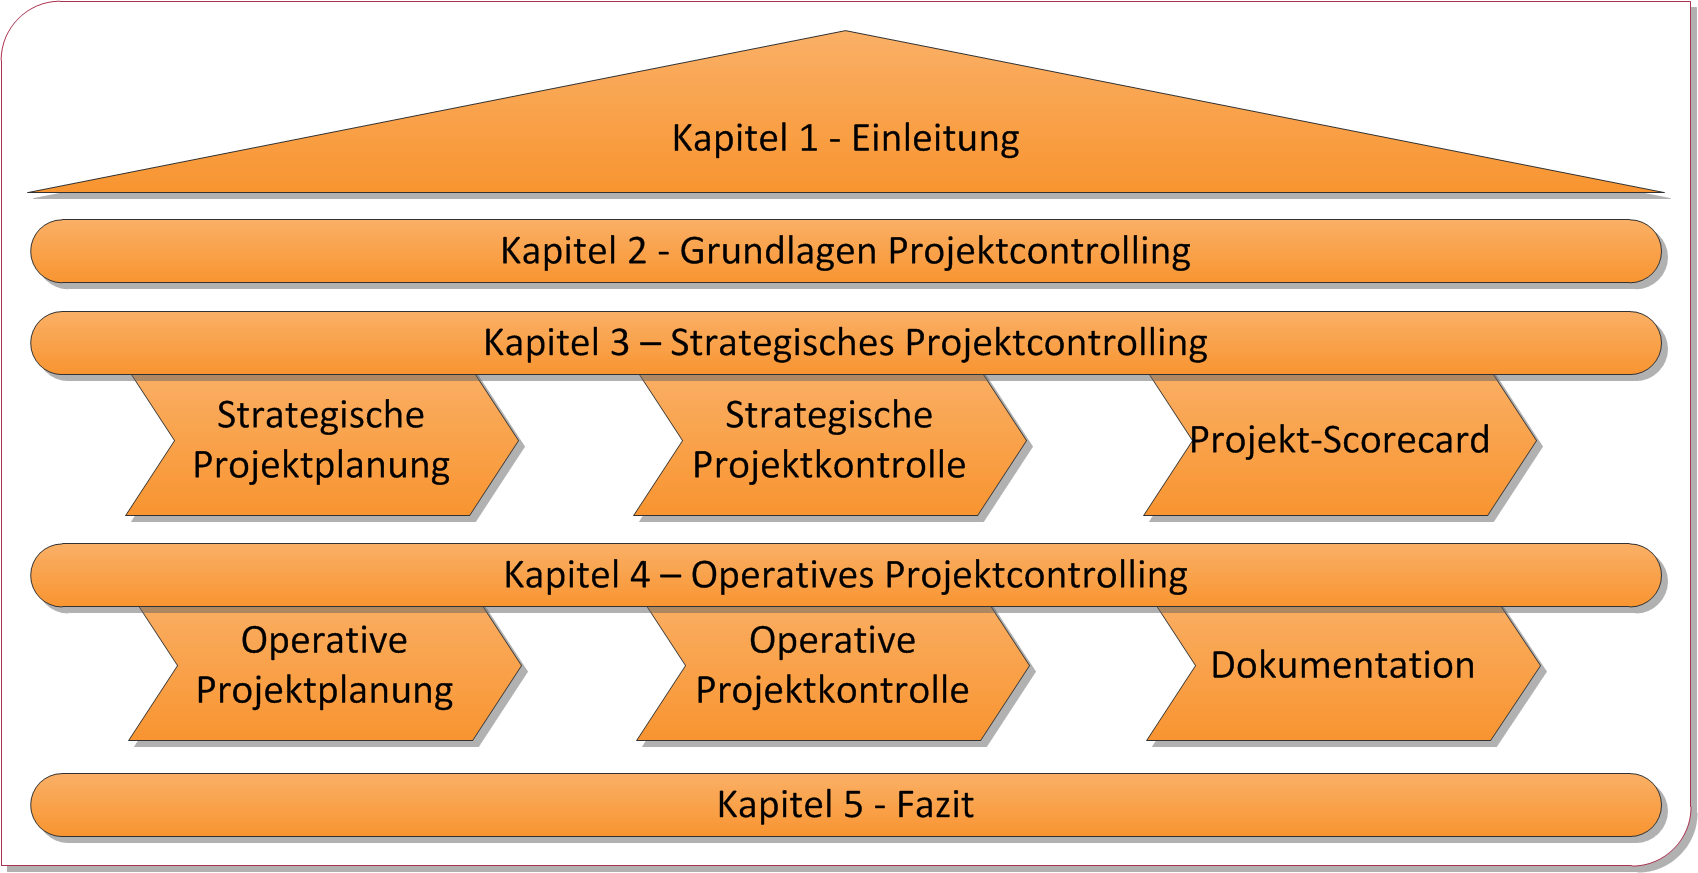
\includegraphics[width=0.8\textwidth]{Images/aufbau.png}
%\caption[Aufbau dieser Arbeit]{Aufbau dieser Arbeit}
%\label{abb1}
%\end{center}
%\end{figure}
%%\end{floatingfigure}
%\begin{compactitem}
%\item Kapitel 1 führt an das betrachtete Thema heran und definiert die Ziele dieser Arbeit.
%\item Kapitel 2 gibt einen Überblick über Projektcontrolling im Projektmanagement. Angesprochen werden die Ausprägungen, sowie die Aufgaben und Ziele des Projektcontrollings.
%\item Kapitel 3 behandelt das Projektcontrolling aus strategischer Sicht. Es wird die Auswahl und Priorisierung von Projekten in einem Projektportfolio erklärt, aber auch um den Einsatz der Project Scorecard für die Projektauswahl und Projektsteuerung.
%\item Kapitel 4 bildet den Schwerpunkt der Arbeit. Es beschreibt das operative Projektcontrolling und orientiert sich an den Lebenszyklusphasen eines Projektes. Die Sicht auf die Planung wird um die Aspekte der Steuerung und Kontrolle ergänzt.
%\item Kapitel 5 [...]tbd
%\end{compactitem}
